\documentclass{article}

\usepackage[margin=1in]{geometry}
\usepackage[T1]{fontenc}
\usepackage[fontsize=11pt]{fontsize}
\usepackage{fancyhdr}
\usepackage{extramarks}
\usepackage{amsmath}
\usepackage{amsthm}
\usepackage{amsfonts}
\usepackage{tikz}
\usepackage[plain]{algorithm}
\usepackage{algpseudocode}
\usepackage{multicol}
\usepackage{hyperref}

\usetikzlibrary{automata,positioning}

\linespread{1}

\pagestyle{fancy}
\lhead{\hmwkAuthorName}
\chead{\hmwkClass: \ \paprTitle}
\rhead{\today}
\lfoot{\hmwkTitle}
\cfoot{\thepage}

\renewcommand\headrulewidth{0.25pt}
\renewcommand\footrulewidth{0.25pt}

\setlength\columnseprule{.25pt}
\setlength{\columnsep}{2.5pc}
\setcounter{secnumdepth}{0}


\newcommand{\hmwkTitle}{Assignment\ \#6}
\newcommand{\paprTitle}{\\ Future Social Computing - Internet Auction House}
\newcommand{\hmwkDueDate}{June 15, 2023 @ 23:59, EST}
\newcommand{\hmwkClass}{CIS 517 - Social Computing}
\newcommand{\hmwkAuthorName}{\textbf{Cason Konzer}}


\title{
    \vspace{2in}
    \textmd{\textbf{\hmwkClass:\ \\ \hmwkTitle}}\\
    \normalsize\vspace{0.1in}\small{Due\ on\ \hmwkDueDate}\\
    \vspace{0.1in}\Large{\textit{\paprTitle}}
    \vspace{3in}
}

\author{\hmwkAuthorName}
\date{\today}

\begin{document}

\maketitle

\pagebreak

% \tableofcontents
% \listoftables
% \listoffigures
\newpage


\section{Proposal}
Internet is sold to consumers today as a subscription service, traditionally contractual and billed monthly. 
Often times consumers do not use their purchased subscription in whole, yet their payment is steady. 
Taking other utility companies as an example, pay per use is a common model. 
Additionally, we see today variable rates such as those implemented in peak hours for power companies. 
As we strive towards a more sustainable future, we must adapt to become more efficient and environmentally conscious in all aspects of life. 
By 2030, predictions expect information and communications technology to use over 20\% of global electricity demand with networks alone accounting for nearly half the demand \cite{Jones_2018}.

The scope of this proposal can be seen as an extension of smart grid privacy assured bidding \cite{7812774} to internet services.
In such a manner, providers tailor a demand response program in which they auction bandwidth allocations to clients. 
Auctions would be held in a set interval where clients bid for a dedicated service until the next auction occurs. 
It is not required that auctions are held in a uniform manner, for example hourly, daily, and monthly auctions could be ran in a parallel and overlapping fashion. 
Under such a system, traditional home consumers may be overwhelmed, finding it complex, while corporations could significantly cut costs and reduce their carbon footprint. 

From the client side, fixed and/or relative price caps could be instantiated for their bids.
The implementation can be envisioned as a partitioning of network infrastructure by ISPs (Internet Service Providers) to standard and governed switches \ref{fig:IAH}.
Implementation may be seen as an `Internet Auction House' where governed switches act as brokers managed by the ISPs.
Governed switches are to be bundled in fashion and interconnected, with a clear hierarchy. 
Under the hierarchy, an Intelligent Platform Management Interface links parents to their children.
Properly structured, switches can scale in accordance with demand, rather than sitting idle. 

Placing the proposal in context of smart grid demand response programs, power and internet bids can be sent together. 
Aggregating the client-side demand, ISPs become enabled to intelligently place their own power bids. 
With respect to privacy, the Internet Auction House itself need not be managed solely by the ISP, but may take place in a distributed fashion. 
Governance switches should be know to standard switches and could be registered in such a fashion. 
In a global context, complexity arises as bandwidth is allocated between regions; partitioning must take place to ensure bandwidth is allocated as required from the client to the target data providers.
Here, it may be required to have bids registered regionally, for instance, a Michigan resident retrieving data from Ann Arbor should pay less that if they were to retrieve and equal amount from Japan. 

While futuristic, this proposal is not so far reached. 
Today, similar systems are proposed for power distribution, and are very well on the horizon for ISPs.
A scalable systems as proposed, brings us one step closer to sustainable connectivity. 

\newpage

\section{Appendix : Figures}

\begin{figure}[ht!]
    \centering
    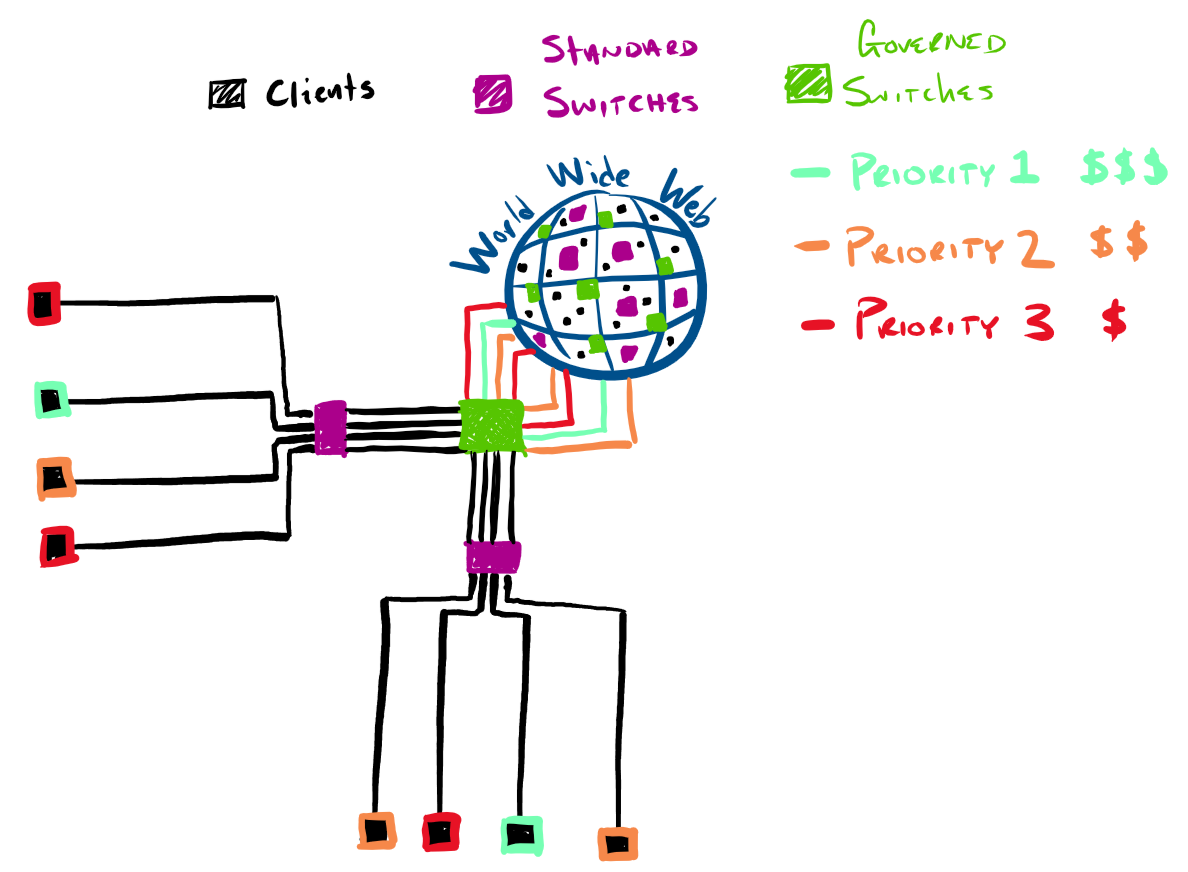
\includegraphics[width=\textwidth]{./Governance.PNG}
    \caption{An abstract view of the Internet Auction House.}
    \label{fig:IAH}
\end{figure}



\newpage

\bibliography{./konzer_cason_CIS_517_assignment_6.bib}{}
\bibliographystyle{naturemag} % abbrv, acm, alpha, apalike, ieeetr, plain, siam, unsrt, tugboat, perception, munich, naturemag
\end{document}